\listfiles


\documentclass[fontsize=11pt,paper=a4,pagesize=auto]{report}

\usepackage{lmodern}
\usepackage[english]{babel}
\usepackage{blindtext}
\usepackage{microtype}
\usepackage{comment, subfiles, graphicx, caption, longtable, subfig, fancyhdr}
\usepackage{float} %Used to force image to appear in the section in which it's declared
\usepackage[hidelinks]{hyperref}
\usepackage[parfill]{parskip}
\usepackage[dvipsnames]{xcolor}
\usepackage{listings}
\usepackage{alloy-style}
\usepackage{xurl}


\makeatletter
\def\p@subsection{}
\makeatother
\begin{document}

\begin{titlepage}
	\centering
	
\includegraphics[scale = 0.20]{images/polimi.jpg}\par
	{\scshape\Large
		Software Engineering 2 Project\\
		a.y. 2020-21\par}
			\vspace{0.5cm}
		
\includegraphics[width=80pt]{images/CLup_logo.png}\par
	{\huge\bfseries
		Customers Line-up\\\par}

	{\Large\bfseries
		Requirements Analysis and Specifications Document\par}
	Version 1.1\par
	\vspace{1cm}
	{\Large
		{\scshape Banfi}  Stefano Alessandro\\
		{\scshape Bresciani} Matteo\par}
	\vfill
	Referent professor: {\scshape Di Nitto} Elisabetta\par
	\vfill
% Bottom of the page
	{\large\today\par}
\end{titlepage}


\tableofcontents
\chapter{Introduction}
\section{Purpose}
\subsection{General Purpose}

The main scope of this document is to define requirements for the application development, in order to make a correct project planification.
\par
To do this, we will analyze:

\begin{itemize}
\item system;
\item functional and unfunctional requirements;
\item constraints;
\item relationships between stakeholders;
\item possible scenarios and tests;
\end{itemize}
\bigskip
These will be shown using different languages such as Alloy and UML.
Then, we will define the context in which our application will be developed.\\
During Sars-Cov-2 emergency, several countries imposed the lockdown in order to hinter the virus diffusion.
People had to change their habits, in fact they could go out only for necessary needs, such as going to the market or pharmacy.\\
For instance people must pay attention while they're entering in the market due to the long queue, which could increase the possibility of virus diffusion.
This fact obliged people to stay for a long time standing up and waiting their turn losing a lots of time. 
\pagebreak

\subsection{Goals}

This are the goals:

\begin{description}
    \item[G1]User enters once arrived at the market.
    \item[G2]Put a limit to the number of Users in the market.
    \item[G3]Smart User can make a Reservation of a seat in the market's queue.
    \item[G4]Smart User can book in advance a Visit in the market.
    \item[G5]Mobile User can make a Reservation of a seat in the market's queue.
    \item[G6]Mobile User can book in advance a Visit in the market.
    \item[G7]Smart User can cancel a booking which can be either a Visit or a Reservation.
    \item[G8]Mobile User can cancel a booking which can be either a Visit or a Reservation.
\end{description}


 
\section{Scope}

The aim of the project is to develop an application which, thanks to an intuitive interface, will avoid customers waiting outside the market.
In order to do that we offer customers three grocery shopping option: 

\begin{itemize}
\item \textbf{Visit}: it's a planned appointment with given date and range time;
\item \textbf{Reservation}: it consits in reserving a virtual seat in market's queue;
\item \textbf{Direct Entrance}: it allows aged customers to enter without any bookings;
\end{itemize}
\bigskip
The main options shown in this documents are the first two in order to avoid customers to line up outside the market. Those are avaiable only for \textbf{Smart} and \textbf{Mobile Users} (their definitions are in subsection 1.3.1).\par
In particular, in order to avoid to wait in line, Users will be allerted by \textbf{notifications} (Smart Users) or a \textbf{SMS} (Mobile Users). These inform them about his time schedule required to reach the market in time.
Only for Smart User the application will provide the position in queue and the time to reach the market.\par
An alphanueric string will be provided to Mobile Users for going in and out from the market. This string for Smart User is converted in two-dimensional bar code using the standard QRCode. This must be submitted at the entry of the market.\par
Instead, the third option is only avaiable if an user is older than 65 years old, but with limitations. For instance they can go grocery shopping only in certain days and time slots. \\
In particular the Direct Entrance is avaiable only from Monday to Friday in the range time between 9.00 A.M and 13.00 P.M. The reason for this selection is due the fact that in this ranges there are fewer customers than any other periods because are working hours. \par
This third option is made especially for aged people who don't have even a mobile phone. \par
The 3 provided methods to go shopping in the market are based on research made by \textit{CENSIS} and \textit{Pew Research Center} that shows how many people in Italy own a smartphone, mobilephone or none.\\
As was shown in these two researches, made in 2018, 71\% of italians own a smartphone, the other 20\% own a mobilephone and the remaining 8\% have none of the two.
Considering that most of the people that don't own a smartphone / mobilephone are older than 65 years old, we can cover most of the customers' market with these 3 shopping options.\\
Analyzing the multiple years data, in the future there will be a significant increase of smartphone/phone and so we cover almost the entire population.\par 
Anyway the RASD document is not focused on the third option.\par


\begin{figure}[H]
  \centering
  %\subfloat[Plot 1.]
  {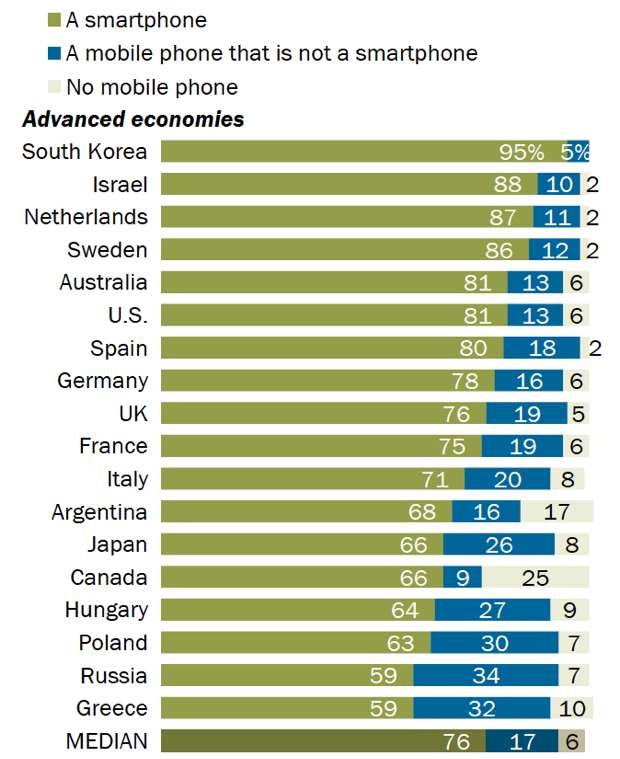
\includegraphics[scale=0.50]{images/statistics_smartphone.png}}
  \hfill
  %\subfloat[Plot 2.]
  {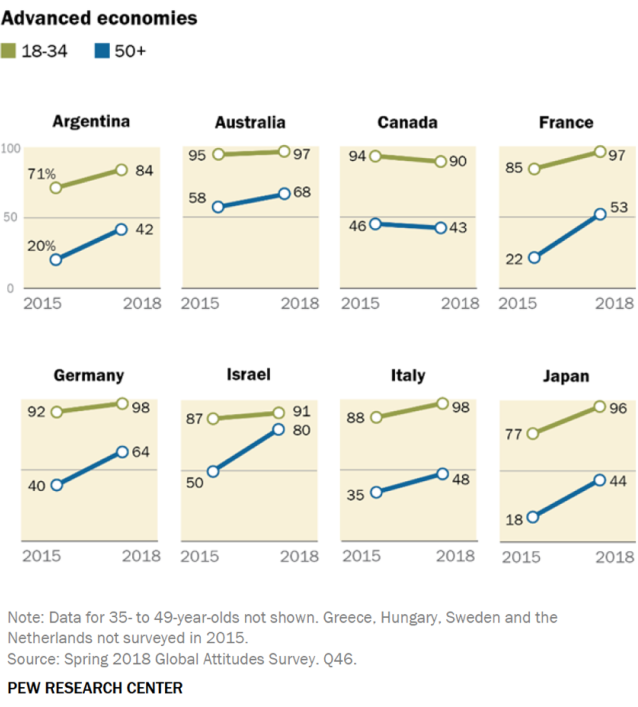
\includegraphics[scale=0.55]{images/statistics_smartphone2.png}\label{fig:f2}}
  \caption{The following charts from Pewresearch website shows percentage of smartphone and mobilephone's owners in each Country.}
\end{figure}

\begin{figure}[H]
  \caption{World and Machine rapresentation.}
  \centering
  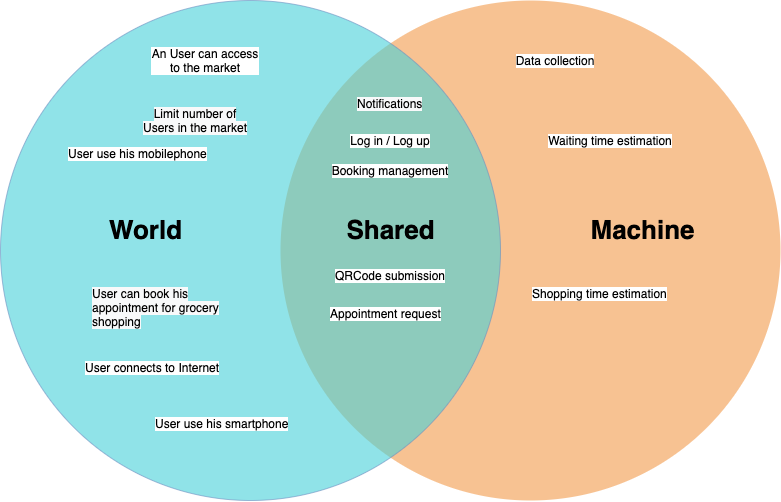
\includegraphics[scale = 0.38]{diagrams/VENN.png}
\end{figure}
\par
\subsection{World}

It represents the environment in which the system is placed. In particular it's composed by events which are affected by the system, but not directly connected with it.
The main \textit{World Phenomena} are:

\begin{itemize}
\item an User can access to the market;
\item limit number of Users in the market;
\item User can book his appointment for grocery shopping;
\item User use his mobilephone / smartphone;
\end{itemize}


\subsection{Machine}
It represents the portion of system to be developed.
The main \textit{Machine Phenomena} are:
\begin{itemize}
\item internal operations;
\item managing any bookings;
\item waiting time estimation;
\item data storage operations;
\end{itemize}
\subsection{Shared Phenomena} 
In this model it needs a common interface to link World and Machine which is composed by the Shared phenomena. \\
Graphically is represent by an intersection between the World and the Machine. In this way World and Machine phenomena are observed from each other.  
The main application Shared Phenomena are the following:
\begin{itemize}
\item Notifications;
\item sign in / sign up;
\item Booking management;
\item QRCode submission;
\item appointment request;
\end{itemize}

\bigskip
\section{Definitions, Acronyms, Abbreviations}
\subsection{Definitions}
\label{info}
\begin{itemize}
\item \textbf{User}: Generic customer who plan to shop in the market. He/she could be a Smart or Mobile User;
\item \textbf{Smart User}: User who has got a smartphone with CLup app. She/He's able to manage bookings by herself/himself;
\item \textbf{Mobile User}: User who hasn't got a smartphone (only mobilephone) and so he's not able to manage Booking by himself. A Mobile User allows a Receptionist to manage his booking by calling a telephone number by interacting with him;
\item \textbf{CLup Operator}: desktop application used by Receptionists to manage bookings of Mobile Users;
\item \textbf{Shopping Size}: it's the size of the grocery shopping. It could be \textit{small}, \textit{medium}, \textit{large} depending on the number of items that users will buy. The duration of the permanence inside the market is based on it; 
\item \textbf{Booking}: it indicates the generic appointment of a User in the market. It could be a Reservation or a Visit;
\item \textbf{Reservation}: it's a type of booking. Users simply book a seat at the market's queue. In addition User have to indicate the Shopping Size; 
\item \textbf{Visit}: it's a Booking planned in advance by Users. It is planned by putting the date and the range time in which the User is going grocery shopping. In addition User have to indicate the Shopping Size; 
\item \textbf{Reader}: it reads QRCode at the market's entrance. It allows User to go in / out;
\item \textbf{Booking submitted}: it means that the QRCode related to it is already submitted in the Reader;
\item \textbf{Visit activated}: it's a Visit which already booked but not yet submitted by the User;
\item \textbf{Reservation activated}: it's a Reservation which already booked but not yet submitted by the User;
\item \textbf{Timestamp}: a digital record of the time of occurrence of a particular event;
\item\textbf{Mirroring}: Mirroring is a technique to allow server to automatically maintain a dual backup of the system;
\end{itemize}

\pagebreak

\begin{itemize}
\subsection{Acronyms}
\item \textbf{RASD}: Requirement Analysis and Specification Document;
\item \textbf{HW}: Hardware;
\item \textbf{SW}: Hardware;
\item \textbf{API}: Application Programming Interface;
\item \textbf{HTTPS}: Hypertext Transfer Protocol Secure;
\item \textbf{DBMS}: Database Management System;
\item \textbf{FOL}: First Order Logic;
\item \textbf{UML}: Unified Modeling Language;


\end{itemize}




\subsection{Abbreviations}
\begin{itemize}
\item \textbf{App}: Application;
\item \textbf{Gn}: n-th goal;
\item \textbf{Rn}: n-th requirement;
\end{itemize}



\section{Revision history}



\section{Reference Documents}
This document is strictly based on:
\begin{itemize}
\item The specification of the \textbf{RASD and DD assignment} of the Software Engineering II corse, held by professor Matteo Rossi and Elisabetta Di Nitto at the Politecnico di Milano, A.Y 2020/2021;
\item \textbf{Slides} of Software Engineering 2 course on BEEP;
\end{itemize}
\section{Document Structure}
Mainly the current document is divided in 4 chapters, which are:
\begin{itemize}
\item[1]\textbf{Introduction}: it aims to describe the environment and the demands taken into account for this project. In particular it's focused on the reasons and the goals that are going to be achieved with its development;
\item[2]\textbf{Overall Description}: it's a high-level description of the system by focusing on the shared phenomena and the domain model (with its assumption); 
\item[3]\textbf{Specific Requirements}: it describes in very detail the requirements needed to reach the goals. In addition it contains more details useful for developers (i.e information about HW and SW interfaces);
\item[4]\textbf{Formal Analysis}: this section contains a formal description of the main aspect of the World phenomena by using Alloy;
\item[5]\textbf{Effort Spent}: it shows the time spent to realize this document, divided for each section;
\item[6]\textbf{References}: it contains the references to any documents and to the Softwares used in this document.
\end{itemize}




\chapter{Overall Description}
\section{Product perspective}

The project aims to build a system that manage the users’ booking (either a Visit or a Reservation) without wasting time while they're waiting their own turn outside the market. 
\par
For a Reservation the system provides User infomation about queue's dynamic in real time (i.e the number of people ahead). 
To do this, the application should try, in the best way, to estimate the time that the customers will spend in the market, in order to notify in advance users who are waiting their own turn outside. 
In addition Users have to indicate how long the shopping time will be, putting potentially the size of the expenditure. This could be Small, Medium or Large.
\\
The application analyses the customers’ statistics and computes the average shopping time.
The calculation considers the time range between the moments in which the User goes in and out.  
\par
In this way, the other customers in queue will be notified as soon as it's the right time to leave and reach the market in time due to the queue's congestion and his position.  

\par
Moreover, it's possible to book a visit choosing the date and the schedule in advance choosing the Visit option. 
\\
The timetable will be splitted into 30 minutes slots, and customers will choose which they want among the free ones. \par

In addition the market will provide costumer, who don't have the application or even a smartphone, a toll-free number in order to make an appointment.
%book a visit or reserve a seat in a virtual queue 
This would be easy-manageble because a receptionist handles the booking and advises the customers with the best shopping option. %as clients' necessary. 
At the beginning, the user will be sign up for booking: so the receptionist will ask the required data from him and will create a customer profile in the system.

The user can also manage (either delete or postpone), in a later moment, hir reservation by calling the same number of the registration.


Once the turn has been called, the user will be noticed through an SMS.
This will contain the identication string that User must show at the entry.

Once the user finished, he will scan the code at the exit to open the doors.


\bigskip
In the UML diagram below will be list the main classes in order to understand how the whole system works.
\par 
\bigskip
\bigskip


\begin{figure}[h]
  \caption{Class diagram with UML}
  \label{fig:UML}
  \centering
  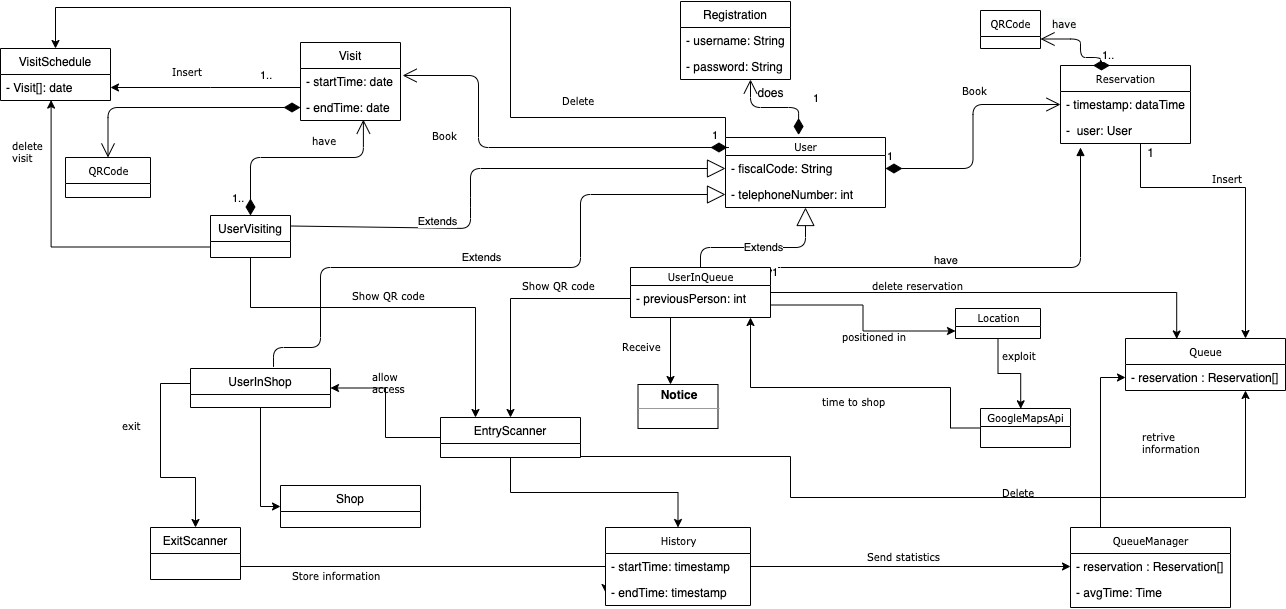
\includegraphics[scale=0.28]{diagrams/UML_simple.png}

\end{figure}
\par 
\medskip
As we can see from the class diagram in figure ~\ref{fig:UML}, the User can book once or a visit or a reservation.
In both cases will be provide him a QRcode, which will be submitted to enter in the market. 
If the the User decided to undo his reservation in the queue could do it by making a cancellation from the application. 
\par
\medskip
In addition the system will notice the User through an SMS or a notice when it's almost his turn (10-15 minutes before).

Now we will analyze the interaction between the User and the system, in order to understand possible criticities.
\par 
\bigskip

\begin{figure}[h]
  \caption{State diagram of the reservation in the queue}
  \label{fig:Reservation}
  \centering
  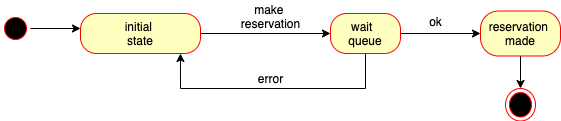
\includegraphics[width=0.8\textwidth, height=0.2\textwidth]{diagrams/2-reservation.png}

\end{figure}
\par 
\medskip

In the  first state diagram (Figure ~\ref{fig:Reservation}) it can be osserved how a generic User can make a reservation thorugh the system. It's sufficient making this action to be added in queue to enter in the market.
\\If something goes wrong the User will be redirect to the initial state.
\\Usually the system reject the request if the market is next to closure (or for logistic problem).

\par 
\medskip

\begin{figure}[h]
  \caption{State diagram of booking a visit}
  \label{fig:Visit}
  \centering
  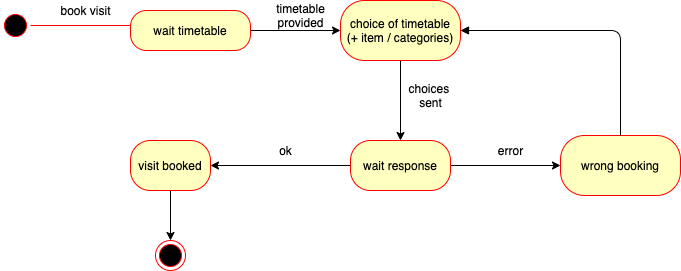
\includegraphics[width=0.8\textwidth, height=0.4\textwidth]{diagrams/2-visit.png}
\end{figure}

\par 
\medskip

The Figure ~\ref{fig:Visit} explains instead how to book a visit in the market. Once the timetable is provided, the generic 



To anticipated the unexpected, the system will use a grace.
Let us assume that we have 100 place into the market, the system will provide only 90 places.
The remaining ten places will be used only for emergency or in the time period in which the customer will enter/exit from the market.
This "grace" will be a userful resource for the system because in this way it will can manage non-deterministic event, like users shopping time, avoiding the market crowding. 
The system will determine the average shopping time according to the information who the user enter when booked the visit/reservation.
In this way, when the shopping time will be near to the average shopping time, the system will notice the first user in queue to reach the supermarket.  
Our goal will be 


User have to select the range time of the visit and the items that he wants to purchase. \par If the choice made by the user is wrong (i.e timetable's slot full), the system notify him; the User will try again until his choice is correct.
\par 
\medskip


\section{Product functions}
\subsection{Queue Manager}
The most important function is the \textit{Queue Manager} because it must avoid the users waiting too much their turn in the case of a wrong use of notifications. [TODO]
In fact, it have to foresee, through statistics from users’ information, the correct time in which the users will enter in the market. This can be done thanks to the notifications sent to the user.
It will also have to decide whether to accept or refuse an appointment, depending on the shop closing time and the number of people in queue. 



To anticipated the unexpected, the system will use a grace.
Let us assume that the maximum number of Users into the market is 100. Well, the system will provide only 90 Users.
The remaining 10 will be used only for emergency or in the time period in which the customer will enter or exit from the market.
This "grace" will be a usefull resource for the system because it can manage non-deterministic event, like user's shopping time %, which is a stochastic prediction.
The system will determine the average shopping time according to the information who the user enter during the Booking.
In particular accuracy of the computation depends on the quality of User's data.
In this way, when the shopping time will be near to the average shopping time, the system will notice the first user in queue to reach the supermarket.  
Our goal is to monitor the User's influx and to keep it under critical boundary (more or less 95). Therefore this could be possibile by flowing slowly the virtual queue.

\subsection{Data Collection}
The \textit{Data Collection} is essential for the correct behavior of the Queue Manager described previously, because it will have to provide precise dates according to client’s information. 
Therefore, the system will have to ask clients precise questions according to keep useful informations for estimating the shopping time into the supermarket, without violating users’ privacy. 
\\
In order to achieve this goal, it needs to oblige the user to register himself in the system and to check the item to allow the processing of his personal data, necessary to reserve virtually the seat in the queue.
\\
One of the possible information asked could be the dimension of the expenses, which can be estimate by the number of item that are going to be purchased. This will be used, with the entry time, to track the number of user inside the market who is finishing. Then will be possibile to notify in advance users in queue about the closeness of their turn.

\section{User characteristics}
We distinguish the actors into our application based on actions and interactions with the external world:

\begin{itemize}
\item \textit{User}: he’s a client who has signed in the system and he can book a visit or take his queue number.
\item \textit{UserInQueue}: he’s a User who has taken his own turn in queue and he’s waiting for the system notification
\item \textit{UserVisiting}: he’s a User who has booked a visit and he’s still waiting for entering into the supermarket.
\item \textit{UserInShop}: he’s a client who has taken his own queue ticket or he has booked a visit. After that he is arrived at the supermarket, he has scanned the QR code and he has entered into the shop.
\end{itemize}


\section{Assumptions, dependencies and constraints}
\subsection{Assumptions}
\begin{description}
    \item[D1] The system delete the Reservation the Smart User accumulates a delay to reach the market greater than 10 minutes
    \item[D2] The system delete the Reservation the Mobile User accumulates a delay to reach the market greater than 15 minutes
    \item[D3] The system handles the threshold number of Users allowed in the market
    \item[D4] The Smart User have to be connected to Internet through Wi-Fi/Cellular network
    \item[D5] The Mobile User have to be connected to Internet through his own mobile operator
    \item[D6] A Visit is associated to a Date and a period of time (start/end time);
    \item[D7] A Booking is associated to one and only one QRCode
    \item[D8] User must have one and only one Visit activated;
    \item[D9] User must have one and only one Reservation activated
    \item[D10] A Booking belongs to one and only one User
    \item[D11] The Waiting Time plus the Shopping Time mustn’t exceed the Closure Time
    \item[D12] In each Date and Slot Time must contain at most N Visits
\end{description}




\chapter{Specific Requirements}
\section{External Interface Requirements}
\subsection{User Interfaces}
\subsection{Hardware Interfaces}
\subsection{Software Interfaces}
\subsection{Communication Interfaces}
\section{Functional Requirements}
Giovanna, a career woman who is always in trouble to find free time, needs to go grocery shopping for her family. 
Indeed, once she finished working, she goes to the market and, due to the lockdown, have to wait in line for hours to have access to it. The result is that, coming back home later, she can't put some time in her children.
However, in the past days, she discovered CLup App which allows her to book a visit in the market in advance, by only putting the range time avaiable and the size of the expenditure.
In this way, Giovanna will save a lot of time and will stay longer with her children, instead of waiting in line outside the market.

Nevertheless, due to Covid-19 emergency, the market will be always filled.

Jonhathan, on the advice of his grandchild, bought a new smartphone.  In addition started using it and installing usefull applications like CLup.
In particular, with it, he'll be able to make a reservation in market's queue. In this way, CLup will notify him when, accordingly to his position, leave to get the market in time for his turn.
Finally, once he arrived, can go in there by simply scanning the QRCode sent before. 
At the end Jonhathan will go shopping without waiting on feet his turn during a cold winter's day.
Gustavo, an elderly person, he discovered recently a new time saver and usefull service at the market. It consists in booking a visit at the market by simply calling the number found in an advertisment. 
Due to the fact that Gustavo is sick of waiting too much in the queue, decides to call this market number to book the visit.
On the other side Marta, a gentle receptionist who works for the market, answers to Gustavo's call; she takes care of the registration of his own data, the credentials and the all visit information (i.e data and range time).

Gustavo will be notified about the appointment with an SMS on his mobilephone in time. In addition the SMS will provide the schedule for the visit and the code which will be submitted at the entrance.



\section{Performance Requirements}
\section{Design Constraints}
\subsection{Standards compliance}
\subsection{Hardware limitations}
\subsection{Any other constraint}

\section{Software System Attributes}
\subsection{Reliability}
\subsection{Availabilitys}
\subsection{Security}
\subsection{Maintainability}
\subsection{Portability}





\chapter{Formal Analysis Using Alloy}
\lstset{language=Alloy}.



\section{Alloy Model}
In this section we show the model of the system, by formalizing it with Alloy. This step is strictly important, due to the consistency of our model. 
In particular it describes the basic structure and the behavior of our system based on FOL.
Our model aims to describe the users's dynamics inside and outside the market in an arbitrary day with their attributes about their bookings.
The main model's aspect described are the following:

\begin{itemize}
\item Users enters in the market with a QRCode if and only if it's valid but not submitted yet. Otherwise, with different boolean values the QRCode signature could have different meaning. All possibile type of QRCode could be:
    \begin{itemize}
    \item \textit{valid and not submitted}: QRCode owner has booked an appointment (either a Reservation or a Visit) and he hasn't entered yet;
    \item \textit{submitted and valid}: the QRCode owner is in the market ;
    \item \textit{submitted and not valid}: the QRCode is already used by the owner;
    \end{itemize}
\item The model is organized temporaly in time slots of 30 minutes each. This way make easier the Visit schedule;
\item The time estimation of each appointment is determined by the bag size. In particular it could be:
\begin{itemize}
\item \textit{Small}: it occupies 1 slot in the schedule, that is 30 minutes;
\item \textit{Medium}: it occupies 2 slots in the schedule, that is 60 minutes;
\item \textit{Large}: it occupies 3 slots in the schedule, that is 90 minutes;
\end{itemize}

\item Users in the queue are put in order depending on his booking number. Smaller is  the booking number higher will be the priority with which the user will enter in the market;

\item Given the timetable of the Visit, only 3 users are allowed to enter in the market with a Visit in the same time. However, this will not formalized in our model due to the fact that it needs a too large number of users in the simulation, which is technically hard for the Alloy tool;

\end{itemize}

\lstinputlisting[language=alloy]{model/alloy.als}




\section{Alloy Results}



\begin{figure}[H]
  \label{marketOpened}
  \centering
  \makebox[\linewidth]{
  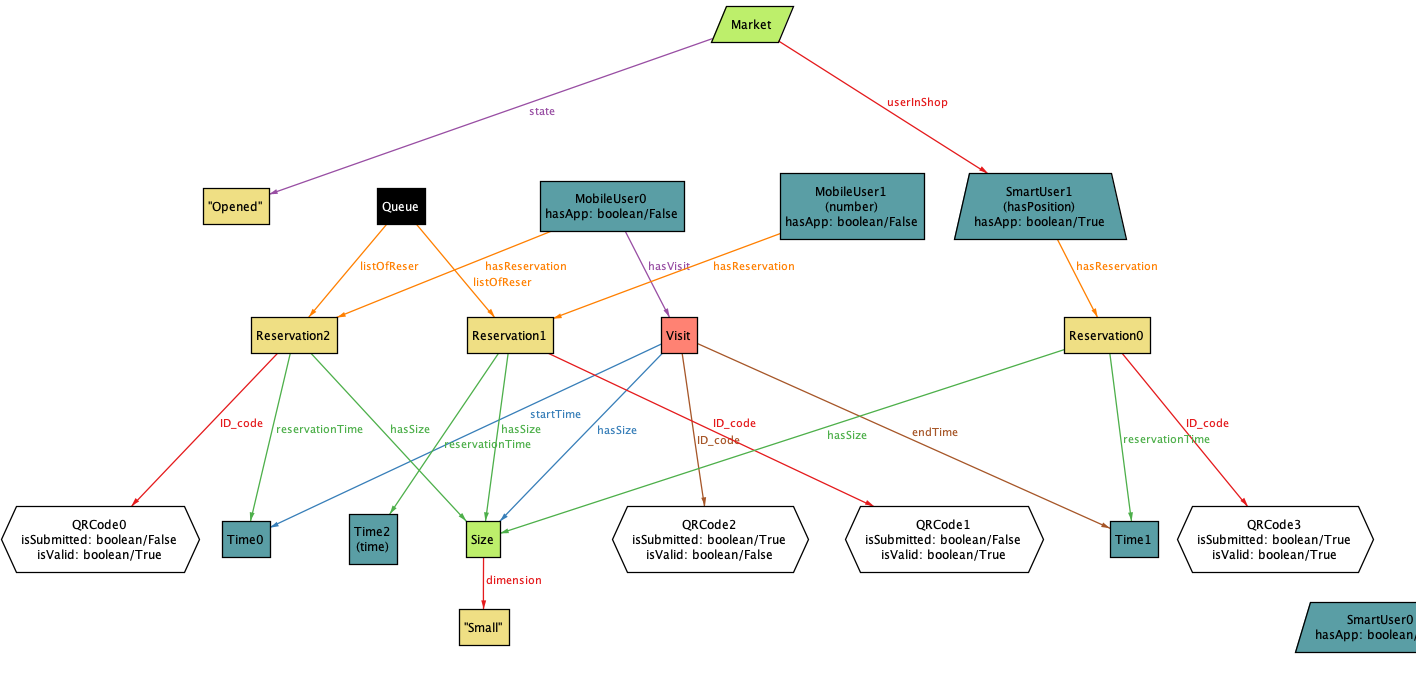
\includegraphics[scale=0.52]{report_alloy/marketOpened.png}}
    \caption{...}
\end{figure}

\begin{figure}[H]
  \label{marketClosed}
  \centering
  \makebox[\linewidth]{
  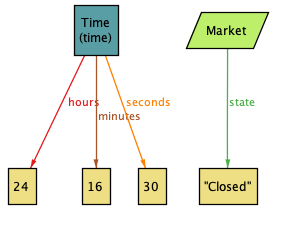
\includegraphics[scale=0.52]{report_alloy/marketClosed.png}}
    \caption{...}
\end{figure}

\begin{figure}[H]
  \label{shorReserv}
  \centering
  \makebox[\linewidth]{
  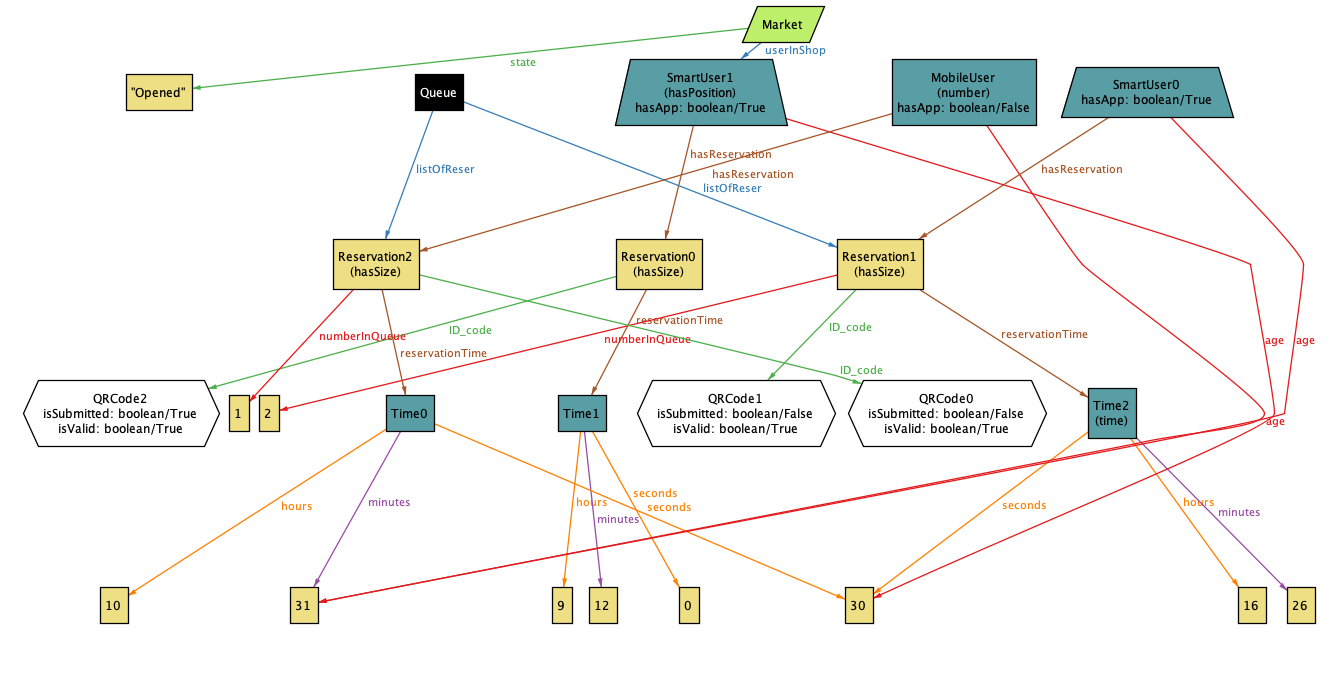
\includegraphics[scale=0.52]{report_alloy/shorReserv.png}}
    \caption{...}
\end{figure}

\begin{figure}[H]
  \label{showVisit}
  \centering
  \makebox[\linewidth]{
  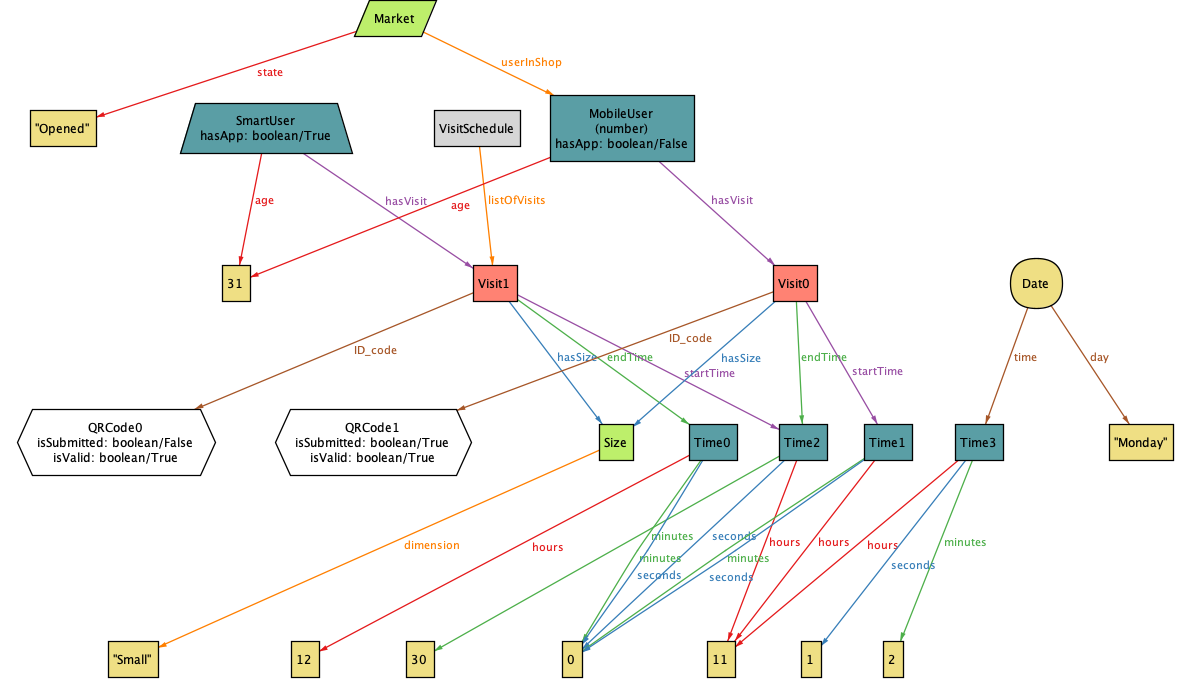
\includegraphics[scale=0.52]{report_alloy/showVisit.png}}
    \caption{...}
\end{figure}


\begin{figure}[H]
  \label{addInQueue}
  \centering
  \makebox[\linewidth]{
  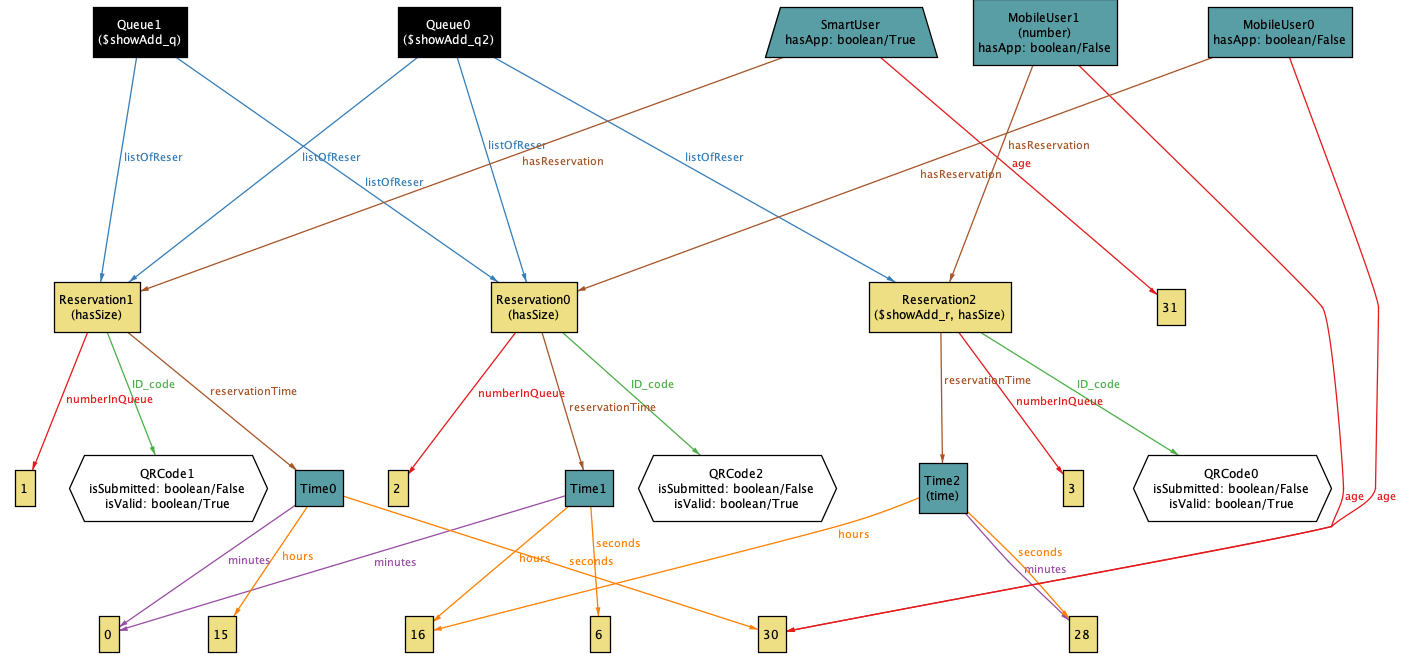
\includegraphics[scale=0.52]{report_alloy/addInQueue.png}}
    \caption{...}
\end{figure}


\begin{figure}[H]
  \label{deInQueue}
  \centering
  \makebox[\linewidth]{
  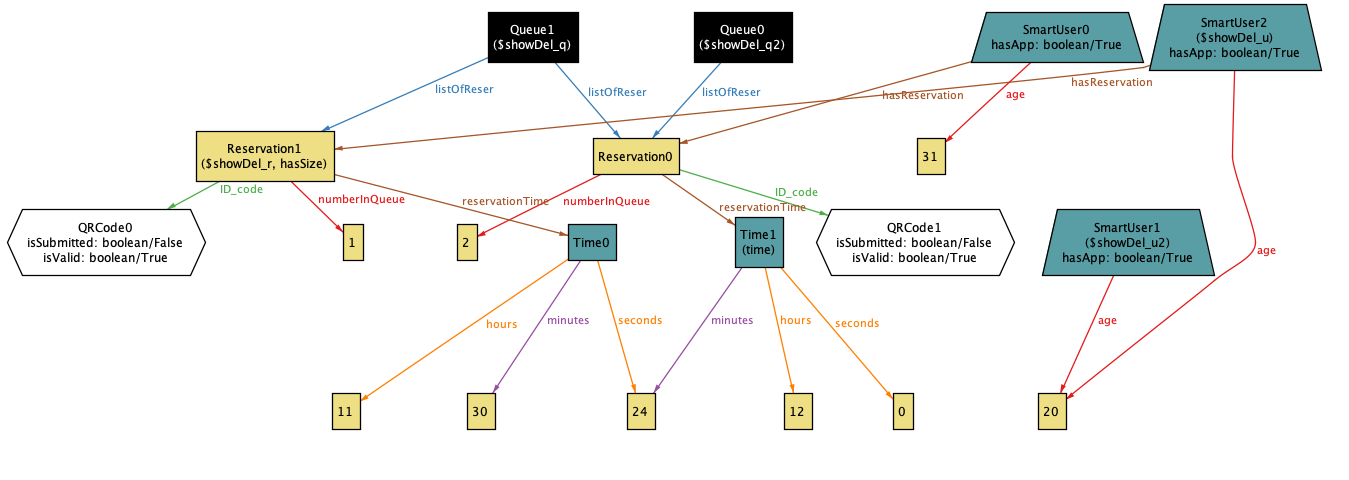
\includegraphics[scale=0.52]{report_alloy/deInQueue.png}}
    \caption{...}
\end{figure}


\begin{figure}[H]
  \label{pred1}
  \centering
  \makebox[\linewidth]{
  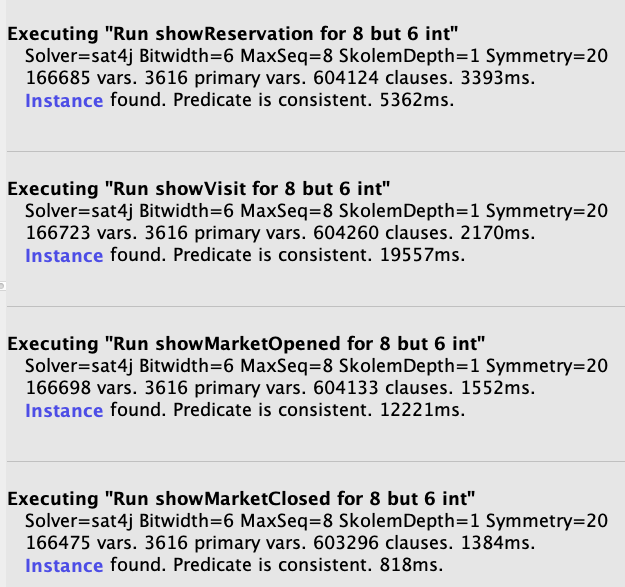
\includegraphics[scale=0.52]{report_alloy/pred1.png}}
    \caption{...}
\end{figure}

\begin{figure}[H]
  \label{pred2}
  \centering
  \makebox[\linewidth]{
  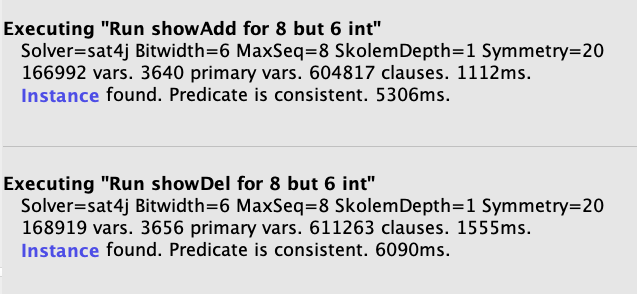
\includegraphics[scale=0.52]{report_alloy/pred2.png}}
    \caption{...}
\end{figure}

\begin{figure}[H]
  \label{reportAssert}
  \centering
  \makebox[\linewidth]{
  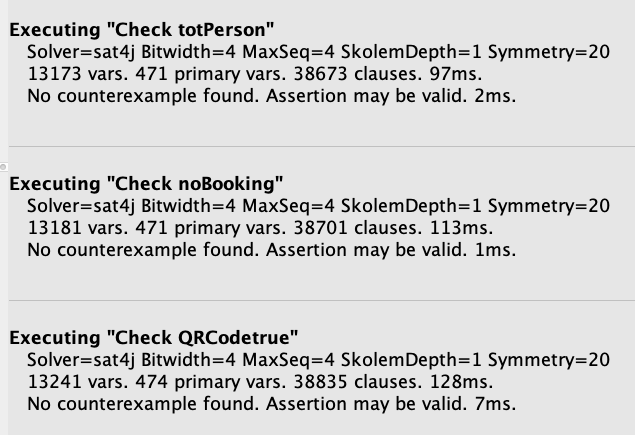
\includegraphics[scale=0.52]{report_alloy/reportAssert.png}}
    \caption{...}
\end{figure}


\chapter{Effort Spent}
In the following tables it's summerized the effort time spent from us. 

	\begin{longtable}{| p{5 cm} | p{1 cm} |} 
			\hline
			{\bf Chapter/Task} & {\bf Hours}\\
			\hline
            Git setup & 1 \\
			Introduction & 6 \\
			Architectural Design & 11 \\
			User Interface Design & 5\\
			Requirements Traceability & 2 \\
			Implementation Integration Test & 1 \\
            Review & 3 \\
			\hline
			&  {\bf Total} \\
			\hline
			&  35 \\
			\hline
			\caption{Matteo Bresciani's effort}
		\end{longtable}

			\begin{longtable}{| p{5 cm} | p{1 cm} |} 
			\hline
			{\bf Chapter/Task} & {\bf Hours}\\
			\hline
			Introduction & 5 \\
			Architectural Design & 11 \\
			User Interface Design & 4 \\
			Requirements Traceability & 2 \\
			Implementation Integration Test & 3 \\
            Review & \\
			\hline
			&  {\bf Total} \\
			\hline
			&  32 \\
			\hline
			\caption{Stefano Banfi's effort}
		\end{longtable}
	


\chapter{References}
\section{Software used}

\begin{itemize}
\item \textbf{\LaTeX}: used to write and to build the document [\url{https://www.draw.io/}];
\item\textbf{Draw}: used to create class, sequence and case diagram [\url{https://www.draw.io/}];
\item\textbf{GitHub}: used to store and manage project repository [\url{https://github.com/}];
\item\textbf{GitHub Desktop}: is the official GitHub application which allows us to contribute to the project repository in an easy way [\url{https://desktop.github.com}];
\item\textbf{Figma}: used to design mockups provided in this document [\url{https://www.draw.io/}];
\begin{comment}
\item\textbf{}:;
\item\textbf{}:;
\item\textbf{}:;
\end{comment}
\end{itemize}



\section{Bibliography}
\begin{itemize}
\item Slides of \textit{Software Engineering 2} course [\url{https://beep.metid.polimi.it/}];
\item \textit{R\&DD Assignment A.Y. 2020-2021} 
[\url{https://beep.metid.polimi.it/}];
\item \textit{AA 2020/2021 Software Engineering 2 - \textit{Requirements Analysis and Specification Document}- Bresciani Matteo, Stefano Alessandro Banfi} 
[\url{}]; 
\item \textit{Oracle DB documentation} 
[\url{https://docs.oracle.com/cd/E24693_01/nav/development.html}]; 
\item \textit{Amazon Web Service documentation} [\url{https://aws.amazon.com/devops/}];
\end{itemize}





\end{document}